
\chapter{Software Design}

\section{Einführung}

\subsubsection{Namespace-Übersicht}
\begin{figure}[h]
    \centering
    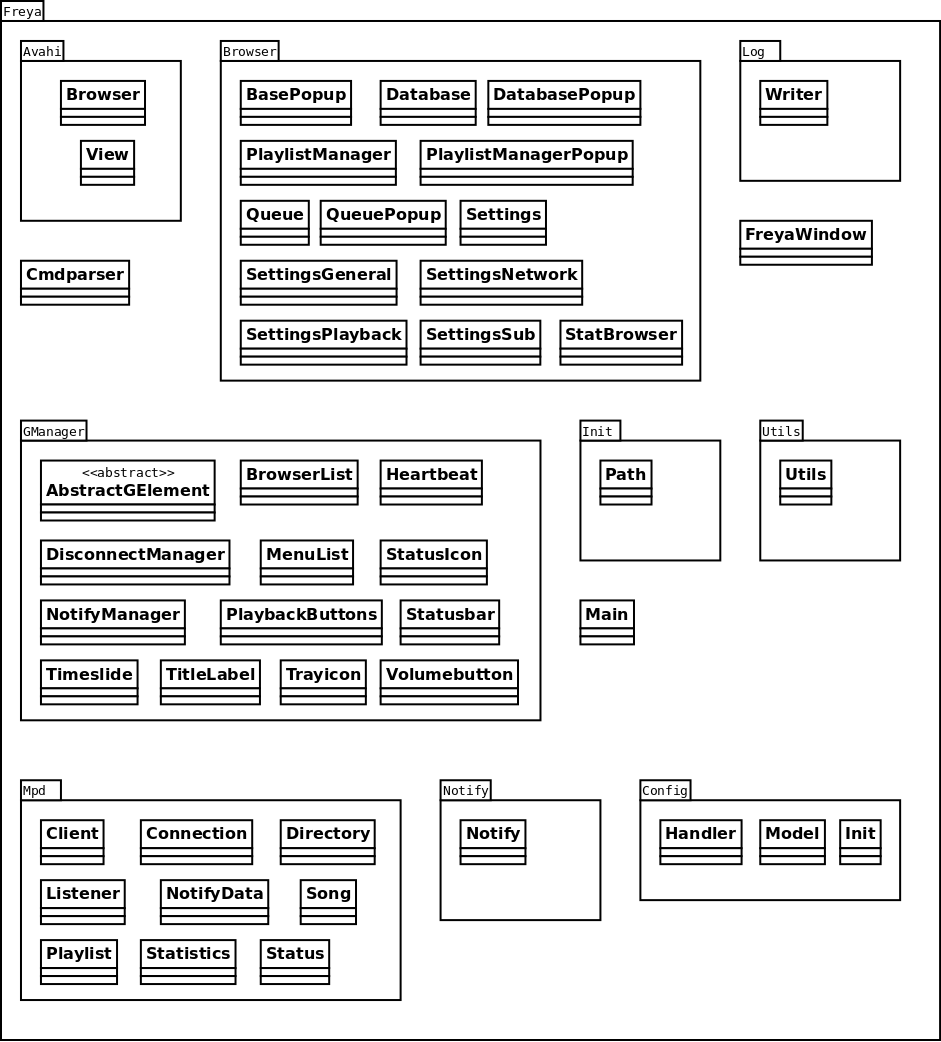
\includegraphics[scale=0.3]{Namespace_Uebersicht.png}
\end{figure}

\section{,,Das Problem''}

Da die grundlegende Funktionsweise des MPD Server auf einer Client Server Architektur beruht, muss der MPD Client
verschiedene Kommandos wie zum Beispiel play, pause, listplaylists etc. an den Server schicken
und zur gleichen Zeit aber auch auf Änderungen reagieren können, d.h. zum Beispiel wenn sich die Lautstärke ändert,
da jederzeit auch andere Clients oder Server den MPD internen Zustand ändern können.
Diese Änderungen müssen auch anderen Programmteilen bekannt gemacht werden. (Observer Pattern)
\\
Der Client sollte im ,,idle''-Mode möglichst keine Ressourcen verschwenden und auch beim 
disconnecten und conntecten die entprechenden Änderungen anderen Teilen des Programms mitteilen
können(Observer Pattern)\footnote{http://de.wikipedia.org/wiki/Observer\_(Entwurfsmuster)}. 
\\

Das MPD Protokoll \footnote{http://www.musicpd.org/doc/protocol/index.html} bietet folgende Möglichkeiten das zu realisieren
\begin{description}
    \item [Periodisch] (zB. alle 500ms) das ,,status'' command absetzen und nach Bedarf auch commands wie ,,currentsong''
        senden
        \\
        \emph{Problem:} Bei langsamen Netzwerkverbindungen erzeugt dies unnötige Netzwerklast 
        Prinzipiell würde sich auf diese Art jedoch die z. B. Musik Bitrate anzeigen lassen, es ist jedoch ein
        wenig komfortabler Weg da hier wieder einmal das Rad neu erfunden werden müsste.
    \item [Nutzung der ,,idle'' und ,,noidle'' commands:]
        ,,idle'' versetzt die Verbindung zum Server in einen Schlafzustand, sobald ,,events'' wie 'player' (also z. B. pause oder play) 
        eintreten, wacht die Verbindung aus diesem Zustand auf und sendet an den Client eine Liste der Events die aufgetreten sind:

\lstinputlisting[language=bash]{state.txt}

        Einschränkung: Während die Verbindung im idle mode ist kann kein reguläres Kommando wie ,,play'' gesendet werden!
        Sollte man es doch tun wird man vom Server augenblicklich mit einem Disconnect belohnt.
        Die einzige Möglichkeit aus dem idle mode aufzuwachen ist das 'noidle' command das gesendet werden
        kann während die verbindung schlafen gelegt wurde.
        Jedoch gibt es auch hier ein Problem, denn das ,,idle'' command blockiert, sprich es sendet kein ,,OK'' zurück zum Sender.
        Ein Warten auf dieses ,,OK'' würde mit den Wunsch eine bedienbare Oberfläche zu haben kollidieren.
\end{description}

Prinzipiell gibt es 2 Möglichkeiten dieses Problem zu lösen:
\begin{itemize}
    \item Man hält zwei Verbindungen zum Server, eine die Kommandos sendet, eine die stets im ,,idle'' mode liegt,
        Für die Realisierung müssten Threads herangezogen werden. Ein Thread würde dann im Hintergrund auf events lauschen,
        der andere würde zum Abschicken der Kommandos benutzt werden.
        Problem: Es müssen 2 Verbindungen gehandelt werden, was wiederum ein Mehraufwand an Code bedeutet.
        Desweiteren werden Threads benötigt die auch in anderen Bereichen des Programms Lockingmechanismen bedeuten würden.
    \item Man hält eine asynchrone verbindung zu dem server.
        Diese kann das 'idle' command zum server schicken, returned aber sofort. Um nun eine Liste der events zu bekommen setzt man 
        einen ,,Watchdog''auf die asynchrone verbindung an (Vergleiche dazu den Systemaufrug 'man 3 poll'). Da poll() ebenfalls den
        aufrufenden Prozess blockiert, wird Glib::signal\_io() benutzt, das sich in den laufenden MainLoop (*) einhängt und eine 
        Callbackfunktion aufruft sobald auf der verbindung etwas interessantes passiert. Da während des Wartens der MainLoop weiterarbeitet,
        bleibt die GUI (und andere Module) aktiv und benutzbar.
        Problem: Vor dem Senden eines Kommandos wie ,,play'' muss der idle mode verlassen werden.
        Lösung: Man kann das ,,noidle'' Kommando zum verlassen senden, und nach dem Absenden des eigentlichen Kommandos wieder den idle-mode betreten.
\end{itemize}

%* MainLoop: Vergleiche Event Dispatcher auf wikipedia. Gtk+ benutzt intern einen MainLoop um auf die user ergebnisse reagieren zu können.
%            Desweiteren kann man eigene events in den Loop einhängen, wie beispielsweise ein Timeoutevent das alle 500ms ausgeführ

\lstinputlisting[language=bash]{telnet.txt}


Die Idee zu dieser Implementierung (speziell das Benutzen einer asynchronen Verbindung), kommt von ,,ncmpc'',
der inoffiziellen offiziellen Referenzimplementierung des MPD Mit-Authors \emph{Max Kellermann}.
Vergleiche \href{http://mpd.wikia.com/wiki/Client:Ncmpc}{ncmpc quellcode}: src/gidle.c und src/mpdclient.c


\section{Aufbau des Clients}
Aus den oben genannten Anforderungen kann eine grobe Architektur abgeleitet werden:

%Hier ein erstes Klassendiagramm zu  
%     * BaseClient
%     * Client 
%     * Connection 
%     * Listener
%     * NotifyData
%bzw. deren Verbindung

\subsection{Hauptklassen}

\subsubsection{BaseClient}
\begin{itemize}
    \item Kann nicht selbst instanziert werden.
    \item Verwaltet connect / disconnect und reconnect vorgänge
    \item Bietet Funktionen zum einfachen verlassen und eintreten des idlemodes an 
    \item Implementiert keine konkreten Kommandos die er an den server schicken kann
    \item Geht die verbindung verloren (ohne dass \emph{disconnect()} explizit aufgerufen wurde),
        so versucht er periodisch sich zu reconnecten.
\end{itemize}

\subsubsection{Listener}
\begin{itemize}
    \item Verwaltet das ein- und austreten aus dem Idlemode
    \item Parst die Responseliste (also changed: player)
    \item Verfügt über ein ,,EventNotifer'' (ein sigc::signal)
        Module können sich über connect() registrieren,
        bemerkt der Listener events so ruft er emit() auf dem signal auf
        und teilt allen anderen Modulen so mit welche events geschehen sind.
    \item Zudem bietet er eine Möglichkeit ein update zur forcen, das heißt ,,künstlich'' alle
        möglichen events auzulösen was nützlich zum Initialisieren ist (force\_update())
    \item Bei einem connect vorgang wird eine Instanz des Listeners instanziert und 
        sofort der idlemodus betreten
    \item Bei einem disconnect wird der Listener gelöscht.
\end{itemize}

\subsubsection{Connection}
\begin{itemize}
    \item Ein Wrapper um die mpd\_connection Struktur von libmpdclient
    \item Ruft letzendlich mpd\_connection\_new() auf 
    \item Bietet eine Schnittstelle um sich über Fehler informieren zu lassen (signal\_error())
    \item Bietet eine get\_connection() methode die bei jedem aufruf prüft ob fehler passiert sind
        In diesem Falle versucht MPD::Connection den Fehler zu bereinigen (falls ein nicht fataler Fehler war).
        Anschließend benachrichtigt MPD::Connection alle module die sich vorher über signal\_error() 
        registriert haben (wie der BaseClient es beispielsweise mit handle\_error() tut)
\end{itemize}

\subsubsection{Client}
\begin{itemize}
    \item Der Client erbt von BaseClient und implementiert konkrete Commandos wie ,,play'',,,random'' etc.
    \item Er bietet zudem Schnittstellen zur Befüllung der Datenbank, der Queue und des Playlistmanagers
    \item Er bietet die Methoden connect() und disconnect() 
    \item Ist in der config ,,settings.connection.autoconnect'' gesetzt so connected er sich automatisch.
    \item Er bietet zudem eine schnittstelle um sich beim listener zu registrieren und im falle von 
        änderungen des connection zustands benachrichtigt zu werden.
\end{itemize}

\subsubsection{NotifyData}
\begin{itemize}
    \item Speichert den Status, den aktuellen Song und die aktuelle Datenbankstatistik
    \item Der Listener...
        \begin{itemize}
            \item instanziert NotifyData im Konstruktor
            \item sagt NotifyData wann er sich updaten soll (update\_all())
            \item gibt eine Referenz auf NotifyData an alle registrierten Module weiter,
                damit diese konkrete Informationen beziehen können.
        \end{itemize}
\end{itemize}


\subsection{Weitere Klassen}
Desweiteren gibt es einige weitere Klassen die am Rande eine Rolle spielen,
und meist Objektorientierte Wrapperklassen für die C-Strukturen von libmpdclient bereitstellen.

\subsubsection{Song}

Die Song Klasse für Wrapper für mpd\_song Struktur und die dazugehörigen Klassen (libmpdclient).
Soll alle Funktionen von libmpdclient \footnote{http://www.musicpd.org/doc/libmpdclient/song\_8h.html} anbieten,
diese werden hier nur aufgelistet aber nicht erklärt da sie genau wie ihre Vorbilder funktionieren:

\begin{verbatim}
    const char * get\_path(void);
    const char * get\_tag(enum mpd\_tag\_type type, unsigned idx);
    unsigned get\_duration(void);
    time\_t get\_last\_modified(void);
    void set\_pos(unsigned pos);
    unsigned get\_pos(void);
    unsigned get\_id(void);
\end{verbatim}


MPD::Song soll zudem eine Funktion bieten um die Metadaten des Songs in einer printf änhlichen Art als String zurückzuliefern:
\begin{verbatim}
    Glib::ustring song\_format(const char* format, bool markup=true);
\end{verbatim}

Ein beispielhafter Aufruf:
\begin{verbatim}
    SomeSong.song\_format("Artist is by \${artist}") 
\end{verbatim}

Die folgenden Tagarten sollen dabei unterstützt werden (sie spiegeln in etwa die mpd\_tag\_type Enumeration von libmpdclient wieder)
\begin{itemize}
    \item artist
    \item title
    \item album
    \item track
    \item name
    \item data
    \item album\_artist
    \item genre
    \item composer
    \item performer
    \item comment
    \item disc
\end{itemize}
Ist ein Escapestring nicht bekannt, so wird er nicht escaped. Ist der tag nicht vorhanden soll mit "unknown" escaped werden.


\subsubsection{Directory}
Die Directory Klasse ist Wrapper für mpd\_directory C-Strukutr. Diese wird als Anzeige für ein Verzeichniss benutzt,
jedoch nicht als Container für andere Elemente.

Entsprechend implementiert bietet MPD::Directory nur:
\begin{verbatim}
    void get_path(void);
\end{verbatim}

Dies ist von der AbstractComposite vorgegeben.


\newpage
\subsubsection{Statistics}
Die Statistics Klasse ist Wrapper für mpd\_stats, implementiert gemäß
\\http://www.musicpd.org/doc/libmpdclient/stats\_8h.html
folgende Funktionen:
\begin{verbatim}
    unsigned get\_number\_of\_artists(void);
    unsigned get\_number\_of\_albums(void);
    unsigned get\_number\_of\_songs(void);
    unsigned long get\_uptime(void);
    unsigned long get\_db\_update\_time(void);
    unsigned long get\_play\_time(void);
    unsigned long get\_db\_play\_time(void);
\end{verbatim}


\subsubsection{Playlist}
Die Playlist Klasse ist Wrapper für die mpd\_playlist Struktur, implementiert von http://www.musicpd.org/doc/libmpdclient/playlist\_8h.html folgende Funktionen:
\begin{verbatim}
    const char * get\_path(void);
    time\_t get\_last\_modified(void);
\end{verbatim}

Bietet desweiteren funktionen zum:
Entfernen der Playlist vom Server (Das Playlistobjekt ist danach invalid):
\begin{verbatim}
    void remove(void);
\end{verbatim}

Laden der Playlist in die Queue:
\begin{verbatim}
    void load(void);
\end{verbatim}

Umbennen der Playlist:
\begin{verbatim}
    void rename(const char * new\_name);
\end{verbatim}

Hinzufügen von Songs zur Playlist:
\begin{verbatim}
    void add\_song(const char * uri);
    void add\_song(MPD::Song& song);
\end{verbatim}

Die genannten Funktionen benötigen müssen den idlemode verlassen können,
daher leitet MPD::Playlist von AbstractClientExtension ab.

\subsubsection{AudioOutput}
Die AudioOutput Klasse ist ein Wrapper für mpd\_output, implementiert von http://www.musicpd.org/doc/libmpdclient/output\_8h.html folgende Funktionen:
\begin{verbatim}
    unsigned get\_id(void);
    const char * get\_name(void);
    bool get\_enabled(void);
\end{verbatim}

Bietet desweiteren funktionen zum:
\begin{itemize}
    \item Enablen des Ausgabegerätes:
        \begin{verbatim}
            bool enable(void);
        \end{verbatim}
    \item Disablen des Ausgabegerätes:
        \begin{verbatim}
            bool disable(void);
        \end{verbatim}
\end{itemize}


Die genannten Funktionen benötigen müssen den idlemode verlassen können,
daher leitet MPD::AudioOutput von AbstractClientExtension ab. 

\subsection{Abstrakte Klassen}
\subsubsection{AbstractClientExtension}
Diese abstrakte Klasse erlaubt abgeleiteten Klasse ähnlich zum BaseClient eigene Kommandos zu implementieren.
Wird von MPD::Playlist und MPD::AudioOutput benutzt
%TODO 


\subsubsection{AbstractClientUser}
\begin{itemize}
    \item Verwaltet einen Pointer auf die MPD::Client Klasse,
        so dass der Anwender der Klasse dies nicht selbst tun muss.
    \item Leitet man ab so müssen folgenden Methoden implementiert werden:
        \begin{verbatim}
            void on\_client\_update(enum mpd\_idle event, MPD::NotifyData& data);
        \end{verbatim}  

        Wird aufgerufen sobald der Listener eine Änderunge feststellt,
        siehe weiter unten "Interaktion des Clients mit anderen Modulen" für eine genauere Erklärung.
        \begin{verbatim}
            void on\_connection\_change(bool server\_changed, bool is\_connected);
        \end{verbatim}

        Wird aufgerufen sobald sich der verbunden/getrennt hat. Im ersten Fall
        ist is\_connected true, im anderen false. Sollte sich der Client verbunden haben,
        und der neue Server entspricht nicht mehr dem neuen so ist auch server\_changed true.
        Dies ist automatisch wahr beim ersten Start.
        Diese werden automatisch durch Ableiten von AbstractClientUser registriert.
        Weiterhin können alle Klassen über den mp\_Client Pointer auf den Client zugreifen.
\end{itemize}


\subsubsection{AbstractItemlist}
Für bestimmte Client funktionen muss eine Nutzerklasse von AbstractItemlist ableiten.
Leitet man ab so muss die Methode add\_item(AbstractComposite * data) implementiert werden. 
Je nach Bedarf kann über dynamic\_cast<Zieltyp*>(data) der entsprechende Datentyp rausgecasted werden.
Beim Aufruf von MPD::Client::fill\_queue ruft der Client die add\_item methode für jeden 
song den er vom server bekommt auf. Die ableitende Klasse kann diese dann verarbeiten.

Dadurch werden alle Methoden von AbstractItemGenerator (bzw. die Klassen die davon ableiten) benutzbar:
\begin{itemize}
    \item fill\_queue
    \item fill\_queue\_changes
    \item fill\_playlists
    \item fill\_ouputs
    \item fill\_filelist
\end{itemize} 

%<Klassendiagramm, bzw. Klassen die es verwenden von Doxygen nehmen>


\subsubsection{AbstractItemGenerator}
Lässt ableitende Klasse folgende Methoden implementieren:
Jede dieser Methoden ruft MPD::Playlist add\_item() von AbstractItemlist auf um ihre Resultate weiterzugeben.

%<Sequenzdiagramm>   
Holt alle Songs der aktuellen Queue.
\begin{verbatim}            
    void fill\_queue(AbstractItemlist& data\_model);
\end{verbatim}

Holt alle geänderten Songs in der Queue seit der Version last\_version. Die Position des ersten geänderten Songs wird in first\_pos gespeichert. 
\begin{verbatim}
    void fill\_queue\_changes(AbstractItemlist& data\_model, unsigned last\_version, unsigned& first\_pos);
\end{verbatim}

Holt alle gespeicherten Playlisten vom Server.
\begin{verbatim}              
    void fill\_playlists(AbstractItemlist& data\_model);
\end{verbatim}

Holt alle Audio Outputs vom Server.
\begin{verbatim}
    void fill\_outputs(AbstractItemlist& data\_model);
\end{verbatim}

Holt alle Songs und Directories aus der Datenbank im Pfad path (nicht rekursiv!)              
\begin{verbatim}
    void fill\_filelist(AbstractItemlist& data\_model, const char * path);
\end{verbatim}

%<Klassendiagramm, bzw. Klassen die es verwenden von Doxygen nehmen>

%-------------------------------------------

\subsubsection{AbstractComposite}
Vereinheitlicht Zugriff auf Komponenten verschiedenen Types.
Die abstrakte Klasse zwingt seine Kinder dazu eine \emph{get\_path()} zu implementieren die die Lage im virtuellen Filesystem des Servers angibt.
Der Hauptnutznieser dieser Klasse ist der Databasebrowser, bzw. den dahinter gelagerten Cache Songs und Verzeichnisse gleich zu behandeln.

Die erbende Klasse muss im Konstruktor angeben ob es sich bei der Klasse um ein ,,File'' (\emph{true} für MPD::Song) oder um einen ,,Container'' (\emph{false} für MPD::Directory) handelt.
Diese ,,is\_leaf'' Eigenschaft kann später mit der Funktion \emph{is\_leaf()} abgefragt werden.

% <Klassendiagramm für alle Klassen die von AbstractComposite erben, siehe Doxygen>

%=============================================

%% Übergang zu GUI Zeugs..

\section{Interaktion des Clients mit anderen Modulen}
\begin{itemize}
    \item Die meisten GUI Klassen leiten von AbstractClientUser ab und speichern daher eine Referenz auf eine Instanz von MPD::Client
        Sie können daher Funktionen wie queue\_add() direkt aufrufen.
    \item AbstractClientUser zwingt die abgeleitenden Klassen folgende Funktionen zu implementieren: 
        \begin{verbatim} 
            void on_client_update(mpd_idle event, MPD::NotifyData& data)
            void on_connection_change(bool server_changed, bool is_connected)
        \end{verbatim}

        1) wird aufgerufen sobald der Listener ein Event festgestellt hat. Für jedes eingetretene Event wird 1)
        einmal aufgerufen. 'event' ist dabei eine Enumeration aller möglichen Events, die von libmpdclient 
        vorgegeben werden. %(Siehe auch http://www.musicpd.org/doc/libmpdclient/idle\_8h.html#a3378f7a24c714d7cb1058232330d7a1c)
        'data' ist eine Referenz auf eine Instanz von MPD::NotifyData. Die benutzenden Klassen können mit
        \begin{itemize} 
            \item get\_status() gibt den aktuellen MPD::Status
            \item get\_song() gibt den aktuellen MPD::Song
            \item get\_statistics() gibt die aktuellen MPD::Statistics
        \end{itemize} 
        so bei Änderungen sofort die aktuellen Änderungen auslesen.



        2) on\_connection\_change wird vom Client aufgerufen sobald die Verbindung verloren geht.
        Dabei zeigt der übergebene boolean Wert ,,is\_connected'' an ob man connected wurde, oder disconnected wurde.
        ,,server\_changed'' soll dann anzeigen ob der Server derselbe ist beim zuvor geschehenen Connectvorgang.
        Dies ist beim ersten Start stets wahr. ,,server+\_changed'' kann nicht wahr sein wenn ,,is\_connected'' falsch ist.
    \item Ableitung von den oben beschriebenen abstrakten Klassen AbstractItemlist und AbstractFilebrowser, um alle Funktionen von AbstractItemGenerator nutzen zu können  
\end{itemize}

\section{Config}
\section{GUI Elementklassen} 
\section{Browserimplementierungen}

